% Options for packages loaded elsewhere
% Options for packages loaded elsewhere
\PassOptionsToPackage{unicode}{hyperref}
\PassOptionsToPackage{hyphens}{url}
\PassOptionsToPackage{dvipsnames,svgnames,x11names}{xcolor}
%
\documentclass[
  letterpaper,
  DIV=11,
  numbers=noendperiod]{scrartcl}
\usepackage{xcolor}
\usepackage{amsmath,amssymb}
\setcounter{secnumdepth}{-\maxdimen} % remove section numbering
\usepackage{iftex}
\ifPDFTeX
  \usepackage[T1]{fontenc}
  \usepackage[utf8]{inputenc}
  \usepackage{textcomp} % provide euro and other symbols
\else % if luatex or xetex
  \usepackage{unicode-math} % this also loads fontspec
  \defaultfontfeatures{Scale=MatchLowercase}
  \defaultfontfeatures[\rmfamily]{Ligatures=TeX,Scale=1}
\fi
\usepackage{lmodern}
\ifPDFTeX\else
  % xetex/luatex font selection
\fi
% Use upquote if available, for straight quotes in verbatim environments
\IfFileExists{upquote.sty}{\usepackage{upquote}}{}
\IfFileExists{microtype.sty}{% use microtype if available
  \usepackage[]{microtype}
  \UseMicrotypeSet[protrusion]{basicmath} % disable protrusion for tt fonts
}{}
\makeatletter
\@ifundefined{KOMAClassName}{% if non-KOMA class
  \IfFileExists{parskip.sty}{%
    \usepackage{parskip}
  }{% else
    \setlength{\parindent}{0pt}
    \setlength{\parskip}{6pt plus 2pt minus 1pt}}
}{% if KOMA class
  \KOMAoptions{parskip=half}}
\makeatother
% Make \paragraph and \subparagraph free-standing
\makeatletter
\ifx\paragraph\undefined\else
  \let\oldparagraph\paragraph
  \renewcommand{\paragraph}{
    \@ifstar
      \xxxParagraphStar
      \xxxParagraphNoStar
  }
  \newcommand{\xxxParagraphStar}[1]{\oldparagraph*{#1}\mbox{}}
  \newcommand{\xxxParagraphNoStar}[1]{\oldparagraph{#1}\mbox{}}
\fi
\ifx\subparagraph\undefined\else
  \let\oldsubparagraph\subparagraph
  \renewcommand{\subparagraph}{
    \@ifstar
      \xxxSubParagraphStar
      \xxxSubParagraphNoStar
  }
  \newcommand{\xxxSubParagraphStar}[1]{\oldsubparagraph*{#1}\mbox{}}
  \newcommand{\xxxSubParagraphNoStar}[1]{\oldsubparagraph{#1}\mbox{}}
\fi
\makeatother

\usepackage{color}
\usepackage{fancyvrb}
\newcommand{\VerbBar}{|}
\newcommand{\VERB}{\Verb[commandchars=\\\{\}]}
\DefineVerbatimEnvironment{Highlighting}{Verbatim}{commandchars=\\\{\}}
% Add ',fontsize=\small' for more characters per line
\usepackage{framed}
\definecolor{shadecolor}{RGB}{241,243,245}
\newenvironment{Shaded}{\begin{snugshade}}{\end{snugshade}}
\newcommand{\AlertTok}[1]{\textcolor[rgb]{0.68,0.00,0.00}{#1}}
\newcommand{\AnnotationTok}[1]{\textcolor[rgb]{0.37,0.37,0.37}{#1}}
\newcommand{\AttributeTok}[1]{\textcolor[rgb]{0.40,0.45,0.13}{#1}}
\newcommand{\BaseNTok}[1]{\textcolor[rgb]{0.68,0.00,0.00}{#1}}
\newcommand{\BuiltInTok}[1]{\textcolor[rgb]{0.00,0.23,0.31}{#1}}
\newcommand{\CharTok}[1]{\textcolor[rgb]{0.13,0.47,0.30}{#1}}
\newcommand{\CommentTok}[1]{\textcolor[rgb]{0.37,0.37,0.37}{#1}}
\newcommand{\CommentVarTok}[1]{\textcolor[rgb]{0.37,0.37,0.37}{\textit{#1}}}
\newcommand{\ConstantTok}[1]{\textcolor[rgb]{0.56,0.35,0.01}{#1}}
\newcommand{\ControlFlowTok}[1]{\textcolor[rgb]{0.00,0.23,0.31}{\textbf{#1}}}
\newcommand{\DataTypeTok}[1]{\textcolor[rgb]{0.68,0.00,0.00}{#1}}
\newcommand{\DecValTok}[1]{\textcolor[rgb]{0.68,0.00,0.00}{#1}}
\newcommand{\DocumentationTok}[1]{\textcolor[rgb]{0.37,0.37,0.37}{\textit{#1}}}
\newcommand{\ErrorTok}[1]{\textcolor[rgb]{0.68,0.00,0.00}{#1}}
\newcommand{\ExtensionTok}[1]{\textcolor[rgb]{0.00,0.23,0.31}{#1}}
\newcommand{\FloatTok}[1]{\textcolor[rgb]{0.68,0.00,0.00}{#1}}
\newcommand{\FunctionTok}[1]{\textcolor[rgb]{0.28,0.35,0.67}{#1}}
\newcommand{\ImportTok}[1]{\textcolor[rgb]{0.00,0.46,0.62}{#1}}
\newcommand{\InformationTok}[1]{\textcolor[rgb]{0.37,0.37,0.37}{#1}}
\newcommand{\KeywordTok}[1]{\textcolor[rgb]{0.00,0.23,0.31}{\textbf{#1}}}
\newcommand{\NormalTok}[1]{\textcolor[rgb]{0.00,0.23,0.31}{#1}}
\newcommand{\OperatorTok}[1]{\textcolor[rgb]{0.37,0.37,0.37}{#1}}
\newcommand{\OtherTok}[1]{\textcolor[rgb]{0.00,0.23,0.31}{#1}}
\newcommand{\PreprocessorTok}[1]{\textcolor[rgb]{0.68,0.00,0.00}{#1}}
\newcommand{\RegionMarkerTok}[1]{\textcolor[rgb]{0.00,0.23,0.31}{#1}}
\newcommand{\SpecialCharTok}[1]{\textcolor[rgb]{0.37,0.37,0.37}{#1}}
\newcommand{\SpecialStringTok}[1]{\textcolor[rgb]{0.13,0.47,0.30}{#1}}
\newcommand{\StringTok}[1]{\textcolor[rgb]{0.13,0.47,0.30}{#1}}
\newcommand{\VariableTok}[1]{\textcolor[rgb]{0.07,0.07,0.07}{#1}}
\newcommand{\VerbatimStringTok}[1]{\textcolor[rgb]{0.13,0.47,0.30}{#1}}
\newcommand{\WarningTok}[1]{\textcolor[rgb]{0.37,0.37,0.37}{\textit{#1}}}

\usepackage{longtable,booktabs,array}
\usepackage{calc} % for calculating minipage widths
% Correct order of tables after \paragraph or \subparagraph
\usepackage{etoolbox}
\makeatletter
\patchcmd\longtable{\par}{\if@noskipsec\mbox{}\fi\par}{}{}
\makeatother
% Allow footnotes in longtable head/foot
\IfFileExists{footnotehyper.sty}{\usepackage{footnotehyper}}{\usepackage{footnote}}
\makesavenoteenv{longtable}
\usepackage{graphicx}
\makeatletter
\newsavebox\pandoc@box
\newcommand*\pandocbounded[1]{% scales image to fit in text height/width
  \sbox\pandoc@box{#1}%
  \Gscale@div\@tempa{\textheight}{\dimexpr\ht\pandoc@box+\dp\pandoc@box\relax}%
  \Gscale@div\@tempb{\linewidth}{\wd\pandoc@box}%
  \ifdim\@tempb\p@<\@tempa\p@\let\@tempa\@tempb\fi% select the smaller of both
  \ifdim\@tempa\p@<\p@\scalebox{\@tempa}{\usebox\pandoc@box}%
  \else\usebox{\pandoc@box}%
  \fi%
}
% Set default figure placement to htbp
\def\fps@figure{htbp}
\makeatother





\setlength{\emergencystretch}{3em} % prevent overfull lines

\providecommand{\tightlist}{%
  \setlength{\itemsep}{0pt}\setlength{\parskip}{0pt}}



 


\usepackage{booktabs}
\usepackage{longtable}
\usepackage{array}
\usepackage{multirow}
\usepackage{wrapfig}
\usepackage{float}
\usepackage{colortbl}
\usepackage{pdflscape}
\usepackage{tabu}
\usepackage{threeparttable}
\usepackage{threeparttablex}
\usepackage[normalem]{ulem}
\usepackage{makecell}
\usepackage{xcolor}
\KOMAoption{captions}{tableheading}
\makeatletter
\@ifpackageloaded{caption}{}{\usepackage{caption}}
\AtBeginDocument{%
\ifdefined\contentsname
  \renewcommand*\contentsname{Table of contents}
\else
  \newcommand\contentsname{Table of contents}
\fi
\ifdefined\listfigurename
  \renewcommand*\listfigurename{List of Figures}
\else
  \newcommand\listfigurename{List of Figures}
\fi
\ifdefined\listtablename
  \renewcommand*\listtablename{List of Tables}
\else
  \newcommand\listtablename{List of Tables}
\fi
\ifdefined\figurename
  \renewcommand*\figurename{Figure}
\else
  \newcommand\figurename{Figure}
\fi
\ifdefined\tablename
  \renewcommand*\tablename{Table}
\else
  \newcommand\tablename{Table}
\fi
}
\@ifpackageloaded{float}{}{\usepackage{float}}
\floatstyle{ruled}
\@ifundefined{c@chapter}{\newfloat{codelisting}{h}{lop}}{\newfloat{codelisting}{h}{lop}[chapter]}
\floatname{codelisting}{Listing}
\newcommand*\listoflistings{\listof{codelisting}{List of Listings}}
\makeatother
\makeatletter
\makeatother
\makeatletter
\@ifpackageloaded{caption}{}{\usepackage{caption}}
\@ifpackageloaded{subcaption}{}{\usepackage{subcaption}}
\makeatother
\usepackage{bookmark}
\IfFileExists{xurl.sty}{\usepackage{xurl}}{} % add URL line breaks if available
\urlstyle{same}
\hypersetup{
  pdftitle={Trabajo Final: Tlaxcala},
  pdfauthor={Nicolas de Silva Nacenta; Emmanuel Escobar Gutierrez},
  colorlinks=true,
  linkcolor={blue},
  filecolor={Maroon},
  citecolor={Blue},
  urlcolor={Blue},
  pdfcreator={LaTeX via pandoc}}


\title{Trabajo Final: Tlaxcala}
\author{Nicolas de Silva Nacenta \and Emmanuel Escobar Gutierrez}
\date{}
\begin{document}
\maketitle


\subsection{\texorpdfstring{\textcolor{violet}{Introducción}}{}}\label{section}

Tlaxcala es el estado más pequeño de México, con \(4016km^2\), ademas
cuenta con \(1,342,977\) personas que residen en el estado, con una
población mayoritariamente femenina con un \(51.6\%\) y ademas de una
edad mediana de aproximadamente \(28\) años, lo cual refleja una
población mayoritariamnete joven

Se estima que la tasa de desempleo del estado es de \(2.54\%\) , la tasa
de participación laboral es de \(60.2\%\) y con un \(70.9\%\) de la
población en un sector informal, tambien sabemos que la esperanza de
vida es de \(75\) años en promedio aunque siendo mayor para las mujeres

A diferencia de otros estados donde la población se concentra en una
sola metrópoli, Tlaxcala presenta un modelo de dispersión urbana. La
población se reparte en una constelación de municipios como Tlaxcala de
Xicohténcatl, Huamantla, San Pablo del Monte y Apizaco, ninguno de los
cuales domina de forma absoluta sobre los demás. Esta estructura plantea
retos únicos en términos de infraestructura, movilidad y acceso a
servicios de salud, donde la cobertura alcanza actualmente al \(71.8\%\)
de los tlaxcaltecas.

\subsection{\texorpdfstring{\textcolor{violet}{Lectura}}{}}\label{section-1}

La demografía es una ciencia social cuantitativa fundamental que nos
permite entender el mundo desde la infancia por el conteo de edades y se
vuelve crucial en la adultez para analizar retos globales como el
envejecimiento, la migración y los cambios en la fertilidad. Esta
disciplina destaca por la simplicidad de sus unidades de análisis, la
regularidad de sus procesos biológicos y su capacidad interdisciplinaria
para colaborar con otras ciencias del comportamiento humano. Para que
sus mediciones tengan valor predictivo o explicativo, la demografía se
apoya en modelos matemáticos que interpretan datos provenientes de
cuatro fuentes principales, los censos, los registros vitales de los
gobiernos, las encuestas por muestreo y las observaciones etnográficas
que profundizan en las motivaciones personales de la población.

\subsection{\texorpdfstring{\textcolor{violet}{Análisis De Tlaxcala}}{}}\label{section-2}

\begin{Shaded}
\begin{Highlighting}[]
\CommentTok{\# 1. Remover los objetos}
\FunctionTok{rm}\NormalTok{(}\AttributeTok{list =} \FunctionTok{ls}\NormalTok{())}

\CommentTok{\# 2. Instalar paquetes }

\FunctionTok{library}\NormalTok{(lubridate)}
\end{Highlighting}
\end{Shaded}

\begin{verbatim}
Warning: package 'lubridate' was built under R version 4.4.3
\end{verbatim}

\begin{verbatim}

Adjuntando el paquete: 'lubridate'
\end{verbatim}

\begin{verbatim}
The following objects are masked from 'package:base':

    date, intersect, setdiff, union
\end{verbatim}

\begin{Shaded}
\begin{Highlighting}[]
\FunctionTok{library}\NormalTok{(data.table)}
\end{Highlighting}
\end{Shaded}

\begin{verbatim}
Warning: package 'data.table' was built under R version 4.4.3
\end{verbatim}

\begin{verbatim}

Adjuntando el paquete: 'data.table'
\end{verbatim}

\begin{verbatim}
The following objects are masked from 'package:lubridate':

    hour, isoweek, isoyear, mday, minute, month, quarter, second, wday,
    week, yday, year
\end{verbatim}

\begin{Shaded}
\begin{Highlighting}[]
\FunctionTok{library}\NormalTok{(ggplot2)}
\end{Highlighting}
\end{Shaded}

\begin{verbatim}
Warning: package 'ggplot2' was built under R version 4.4.3
\end{verbatim}

\begin{Shaded}
\begin{Highlighting}[]
\FunctionTok{library}\NormalTok{(dplyr)}
\end{Highlighting}
\end{Shaded}

\begin{verbatim}
Warning: package 'dplyr' was built under R version 4.4.3
\end{verbatim}

\begin{verbatim}

Adjuntando el paquete: 'dplyr'
\end{verbatim}

\begin{verbatim}
The following objects are masked from 'package:data.table':

    between, first, last
\end{verbatim}

\begin{verbatim}
The following objects are masked from 'package:stats':

    filter, lag
\end{verbatim}

\begin{verbatim}
The following objects are masked from 'package:base':

    intersect, setdiff, setequal, union
\end{verbatim}

\begin{Shaded}
\begin{Highlighting}[]
\FunctionTok{library}\NormalTok{(tidyr)}
\end{Highlighting}
\end{Shaded}

\begin{verbatim}
Warning: package 'tidyr' was built under R version 4.4.3
\end{verbatim}

\begin{Shaded}
\begin{Highlighting}[]
\FunctionTok{library}\NormalTok{(kableExtra)}
\end{Highlighting}
\end{Shaded}

\begin{verbatim}
Warning: package 'kableExtra' was built under R version 4.4.3
\end{verbatim}

\begin{verbatim}

Adjuntando el paquete: 'kableExtra'
\end{verbatim}

\begin{verbatim}
The following object is masked from 'package:dplyr':

    group_rows
\end{verbatim}

\begin{Shaded}
\begin{Highlighting}[]
\FunctionTok{library}\NormalTok{(readxl)}

\CommentTok{\# 3. Descargar tablas de datos}
\NormalTok{pop }\OtherTok{\textless{}{-}} \FunctionTok{fread}\NormalTok{(}\StringTok{"https://repodatos.atdt.gob.mx/CONAPO/proyecciones/00\_Pob\_Mitad\_1950\_2070.csv"}\NormalTok{)}

\CommentTok{\# 4. Exploración de la tabla de población}
\FunctionTok{table}\NormalTok{(pop}\SpecialCharTok{$}\NormalTok{ENTIDAD)}
\end{Highlighting}
\end{Shaded}

\begin{verbatim}

     Aguascalientes     Baja California Baja California Sur            Campeche 
              22220               22220               22220               22220 
            Chiapas           Chihuahua    Ciudad de México            Coahuila 
              22220               22220               22220               22220 
             Colima             Durango          Guanajuato            Guerrero 
              22220               22220               22220               22220 
            Hidalgo             Jalisco              México           Michoacán 
              22220               22220               22220               22220 
            Morelos             Nayarit          Nuevo León              Oaxaca 
              22220               22220               22220               22220 
             Puebla           Querétaro        Quintana Roo     San Luis Potosí 
              22220               22220               22220               22220 
            Sinaloa              Sonora             Tabasco          Tamaulipas 
              22220               22220               22220               22220 
           Tlaxcala            Veracruz             Yucatán           Zacatecas 
              22220               22220               22220               22220 
\end{verbatim}

\begin{Shaded}
\begin{Highlighting}[]
\FunctionTok{table}\NormalTok{(pop}\SpecialCharTok{$}\NormalTok{CVE\_GEO)}
\end{Highlighting}
\end{Shaded}

\begin{verbatim}

    1     2     3     4     5     6     7     8     9    10    11    12    13 
22220 22220 22220 22220 22220 22220 22220 22220 22220 22220 22220 22220 22220 
   14    15    16    17    18    19    20    21    22    23    24    25    26 
22220 22220 22220 22220 22220 22220 22220 22220 22220 22220 22220 22220 22220 
   27    28    29    30    31    32 
22220 22220 22220 22220 22220 22220 
\end{verbatim}

\begin{Shaded}
\begin{Highlighting}[]
\FunctionTok{table}\NormalTok{(pop}\SpecialCharTok{$}\NormalTok{ANIO)}
\end{Highlighting}
\end{Shaded}

\begin{verbatim}

1970 1971 1972 1973 1974 1975 1976 1977 1978 1979 1980 1981 1982 1983 1984 1985 
7040 7040 7040 7040 7040 7040 7040 7040 7040 7040 7040 7040 7040 7040 7040 7040 
1986 1987 1988 1989 1990 1991 1992 1993 1994 1995 1996 1997 1998 1999 2000 2001 
7040 7040 7040 7040 7040 7040 7040 7040 7040 7040 7040 7040 7040 7040 7040 7040 
2002 2003 2004 2005 2006 2007 2008 2009 2010 2011 2012 2013 2014 2015 2016 2017 
7040 7040 7040 7040 7040 7040 7040 7040 7040 7040 7040 7040 7040 7040 7040 7040 
2018 2019 2020 2021 2022 2023 2024 2025 2026 2027 2028 2029 2030 2031 2032 2033 
7040 7040 7040 7040 7040 7040 7040 7040 7040 7040 7040 7040 7040 7040 7040 7040 
2034 2035 2036 2037 2038 2039 2040 2041 2042 2043 2044 2045 2046 2047 2048 2049 
7040 7040 7040 7040 7040 7040 7040 7040 7040 7040 7040 7040 7040 7040 7040 7040 
2050 2051 2052 2053 2054 2055 2056 2057 2058 2059 2060 2061 2062 2063 2064 2065 
7040 7040 7040 7040 7040 7040 7040 7040 7040 7040 7040 7040 7040 7040 7040 7040 
2066 2067 2068 2069 2070 
7040 7040 7040 7040 7040 
\end{verbatim}

\begin{Shaded}
\begin{Highlighting}[]
\FunctionTok{names}\NormalTok{(pop)}
\end{Highlighting}
\end{Shaded}

\begin{verbatim}
[1] "RENGLON"            "ANIO"               "ENTIDAD"           
[4] "CVE_GEO"            "EDAD"               "SEXO"              
[7] "POBLACION"          "ENTIDAD_FEDERATIVA" "FECHA"             
\end{verbatim}

\begin{Shaded}
\begin{Highlighting}[]
\FunctionTok{sum}\NormalTok{(pop}\SpecialCharTok{$}\NormalTok{POBLACION)}
\end{Highlighting}
\end{Shaded}

\begin{verbatim}
[1] 11781123754
\end{verbatim}

\begin{Shaded}
\begin{Highlighting}[]
\CommentTok{\# Filtrar Estado}

\NormalTok{tlx }\OtherTok{\textless{}{-}}\NormalTok{ pop[ENTIDAD }\SpecialCharTok{==} \StringTok{"Tlaxcala"} \SpecialCharTok{\&}\NormalTok{ ANIO }\SpecialCharTok{==} \StringTok{"2026"}\NormalTok{, .(SEXO, EDAD, POBLACION)]}
\NormalTok{tlx}
\end{Highlighting}
\end{Shaded}

\begin{verbatim}
        SEXO  EDAD POBLACION
      <char> <int>     <int>
  1: Hombres     0     12329
  2: Mujeres     0     11886
  3: Hombres     1     12430
  4: Mujeres     1     11984
  5: Hombres     2     12527
 ---                        
216: Mujeres   107         2
217: Hombres   108         2
218: Mujeres   108         1
219: Hombres   109         1
220: Mujeres   109         0
\end{verbatim}

\subsubsection{\texorpdfstring{\textcolor{purple}{Tabla (Piramide)}}{}}\label{section-3}

\begin{Shaded}
\begin{Highlighting}[]
\CommentTok{\# 5. Transformación de datos para la pirámide}
\CommentTok{\# Agrupamos por rangos de 5 años para que coincida con la imagen}
\NormalTok{tlx\_pyramid }\OtherTok{\textless{}{-}}\NormalTok{ tlx }\SpecialCharTok{\%\textgreater{}\%}
  \FunctionTok{mutate}\NormalTok{(}\AttributeTok{EDAD\_GRP =} \FunctionTok{cut}\NormalTok{(EDAD, }
                        \AttributeTok{breaks =} \FunctionTok{c}\NormalTok{(}\FunctionTok{seq}\NormalTok{(}\DecValTok{0}\NormalTok{, }\DecValTok{85}\NormalTok{, }\AttributeTok{by =} \DecValTok{5}\NormalTok{), }\ConstantTok{Inf}\NormalTok{), }
                        \AttributeTok{labels =} \FunctionTok{c}\NormalTok{(}\StringTok{"0{-}4"}\NormalTok{, }\StringTok{"5{-}9"}\NormalTok{, }\StringTok{"10{-}14"}\NormalTok{, }\StringTok{"15{-}19"}\NormalTok{, }\StringTok{"20{-}24"}\NormalTok{, }\StringTok{"25{-}29"}\NormalTok{, }
                                   \StringTok{"30{-}34"}\NormalTok{, }\StringTok{"35{-}39"}\NormalTok{, }\StringTok{"40{-}44"}\NormalTok{, }\StringTok{"45{-}49"}\NormalTok{, }\StringTok{"50{-}54"}\NormalTok{, }\StringTok{"55{-}59"}\NormalTok{, }
                                   \StringTok{"60{-}64"}\NormalTok{, }\StringTok{"65{-}69"}\NormalTok{, }\StringTok{"70{-}74"}\NormalTok{, }\StringTok{"75{-}79"}\NormalTok{, }\StringTok{"80{-}84"}\NormalTok{, }\StringTok{"85+"}\NormalTok{), }
                        \AttributeTok{right =} \ConstantTok{FALSE}\NormalTok{)) }\SpecialCharTok{\%\textgreater{}\%}
  \FunctionTok{group\_by}\NormalTok{(SEXO, EDAD\_GRP) }\SpecialCharTok{\%\textgreater{}\%}
  \FunctionTok{summarise}\NormalTok{(}\AttributeTok{POBLACION =} \FunctionTok{sum}\NormalTok{(POBLACION)) }\SpecialCharTok{\%\textgreater{}\%}
  \FunctionTok{ungroup}\NormalTok{()}
\end{Highlighting}
\end{Shaded}

\begin{verbatim}
`summarise()` has grouped output by 'SEXO'. You can override using the
`.groups` argument.
\end{verbatim}

\begin{Shaded}
\begin{Highlighting}[]
\CommentTok{\# Convertimos la población de "Hombres" en negativa para el efecto espejo}
\NormalTok{tlx\_pyramid }\OtherTok{\textless{}{-}}\NormalTok{ tlx\_pyramid }\SpecialCharTok{\%\textgreater{}\%}
  \FunctionTok{mutate}\NormalTok{(}\AttributeTok{POBLACION\_GRAF =} \FunctionTok{ifelse}\NormalTok{(SEXO }\SpecialCharTok{==} \StringTok{"Hombres"}\NormalTok{, }\SpecialCharTok{{-}}\NormalTok{POBLACION, POBLACION))}

\CommentTok{\# 6. Generar la gráfica con ggplot2}
\FunctionTok{ggplot}\NormalTok{(tlx\_pyramid, }\FunctionTok{aes}\NormalTok{(}\AttributeTok{x =}\NormalTok{ EDAD\_GRP, }\AttributeTok{y =}\NormalTok{ POBLACION\_GRAF, }\AttributeTok{fill =}\NormalTok{ SEXO)) }\SpecialCharTok{+}
  \FunctionTok{geom\_col}\NormalTok{() }\SpecialCharTok{+}
  \FunctionTok{coord\_flip}\NormalTok{() }\SpecialCharTok{+} \CommentTok{\# Voltea la gráfica para que las barras sean horizontales}
  \FunctionTok{scale\_y\_continuous}\NormalTok{(}\AttributeTok{labels =}\NormalTok{ abs) }\SpecialCharTok{+} \CommentTok{\# Muestra valores absolutos (sin el signo menos)}
  \FunctionTok{scale\_fill\_manual}\NormalTok{(}\AttributeTok{values =} \FunctionTok{c}\NormalTok{(}\StringTok{"Hombres"} \OtherTok{=} \StringTok{"\#a651a1"}\NormalTok{, }\StringTok{"Mujeres"} \OtherTok{=} \StringTok{"\#009688"}\NormalTok{)) }\SpecialCharTok{+} \CommentTok{\# Colores de tu imagen}
  \FunctionTok{theme\_minimal}\NormalTok{() }\SpecialCharTok{+}
  \FunctionTok{labs}\NormalTok{(}\AttributeTok{title =} \StringTok{"Población De Tlaxcala (2026)"}\NormalTok{,}
       \AttributeTok{subtitle =} \StringTok{"Distribución por edad y sexo"}\NormalTok{,}
       \AttributeTok{x =} \StringTok{"Grupos de Edad"}\NormalTok{, }
       \AttributeTok{y =} \StringTok{"Población"}\NormalTok{,}
       \AttributeTok{fill =} \StringTok{"Sexo"}\NormalTok{) }\SpecialCharTok{+}
  \FunctionTok{theme}\NormalTok{(}\AttributeTok{legend.position =} \StringTok{"bottom"}\NormalTok{)}
\end{Highlighting}
\end{Shaded}

\pandocbounded{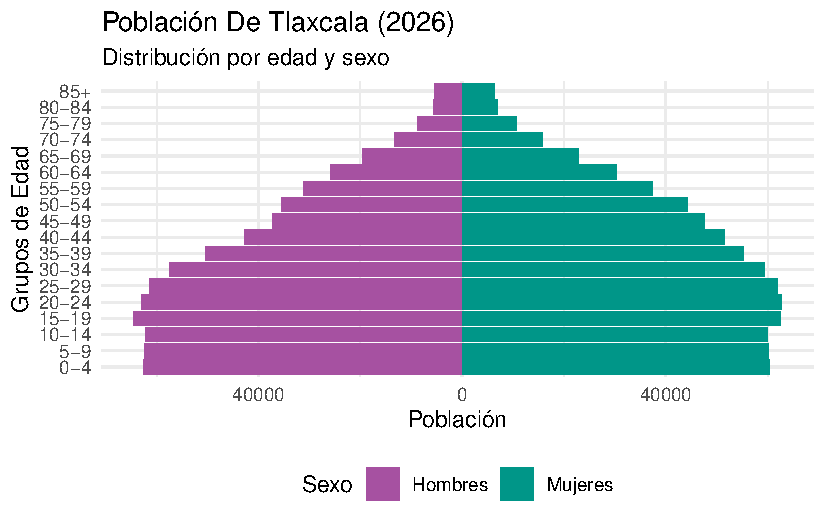
\includegraphics[keepaspectratio]{Trabajo-Final-9219_files/figure-pdf/unnamed-chunk-2-1.pdf}}

The \texttt{echo:\ false} option disables the printing of code (only
output is displayed).

\subsection{\texorpdfstring{\textcolor{violet}{Lectura De La Tabla}}{}}\label{section-4}

La pirámide de Tlaxcala al \(2026\) revela una transición demográfica en
la que el estrechamiento de la base \((0-9 \text{ años})\) refleja una
caída en la natalidad, desplazando el mayor peso poblacional hacia el
lado de los jóvenes de entre \(15\) y \(29\) años. Este perfil indica
que el estado cuenta actualmente con su mayor capacidad de fuerza
productiva, aunque el ensanchamiento visible en los rangos de edades
medias confirma un proceso de envejecimiento gradual de la población,
todo bajo una distribución donde las mujeres representan el \(51.6\%\)
del total debido a su mayor esperanza de vida frente al \(48.4\%\) de
los hombres.

\subsection{}\label{section-5}

\begin{Shaded}
\begin{Highlighting}[]
\NormalTok{(deaths }\OtherTok{\textless{}{-}} \FunctionTok{fread}\NormalTok{(}\StringTok{"data/Mx\_ARG\_GUA.csv"}\NormalTok{))}
\end{Highlighting}
\end{Shaded}

\begin{verbatim}
     year  location     x     D       N
    <int>    <char> <int> <int>   <int>
 1:  2018 Guatemala     0  4888  217902
 2:  2018 Guatemala     1  1325  829069
 3:  2018 Guatemala     5   400  995322
 4:  2018 Guatemala    10   616  991556
 5:  2018 Guatemala    15  1448  973852
 6:  2018 Guatemala    20  2415  880664
 7:  2018 Guatemala    25  2842  757838
 8:  2018 Guatemala    30  2758  631144
 9:  2018 Guatemala    35  2445  526957
10:  2018 Guatemala    40  2054  405425
11:  2018 Guatemala    45  1901  307465
12:  2018 Guatemala    50  2065  240191
13:  2018 Guatemala    55  2785  196290
14:  2018 Guatemala    60  3705  168446
15:  2018 Guatemala    65  4512  132438
16:  2018 Guatemala    70  4766   90297
17:  2018 Guatemala    75  5317   68676
18:  2018 Guatemala    80  5538   45989
19:  2018 Guatemala    85  4366   23775
20:  2018 Guatemala    90  2141    7963
21:  2018 Guatemala    95   593    1697
22:  2018 Argentina     0  4170  384511
23:  2018 Argentina     1   743 1524362
24:  2018 Argentina     5   369 1865386
25:  2018 Argentina    10   487 1818367
26:  2018 Argentina    15  1941 1784875
27:  2018 Argentina    20  2848 1775900
28:  2018 Argentina    25  2673 1745555
29:  2018 Argentina    30  2620 1611697
30:  2018 Argentina    35  2856 1549232
31:  2018 Argentina    40  3534 1444831
32:  2018 Argentina    45  4668 1204426
33:  2018 Argentina    50  7107 1073395
34:  2018 Argentina    55 11153  977548
35:  2018 Argentina    60 15155  856358
36:  2018 Argentina    65 19813  722610
37:  2018 Argentina    70 22172  545982
38:  2018 Argentina    75 23019  362715
39:  2018 Argentina    80 22301  221552
40:  2018 Argentina    85 17000  113250
41:  2018 Argentina    90  8340   39765
42:  2018 Argentina    95  2542    9356
     year  location     x     D       N
    <int>    <char> <int> <int>   <int>
\end{verbatim}

\begin{Shaded}
\begin{Highlighting}[]
\FunctionTok{kable}\NormalTok{(deaths, }\AttributeTok{caption=} \StringTok{"Muertes de Argentina y Guatemala"}\NormalTok{) }
\end{Highlighting}
\end{Shaded}

\begin{longtable}[]{@{}rlrrr@{}}
\caption{Muertes de Argentina y Guatemala}\tabularnewline
\toprule\noalign{}
year & location & x & D & N \\
\midrule\noalign{}
\endfirsthead
\toprule\noalign{}
year & location & x & D & N \\
\midrule\noalign{}
\endhead
\bottomrule\noalign{}
\endlastfoot
2018 & Guatemala & 0 & 4888 & 217902 \\
2018 & Guatemala & 1 & 1325 & 829069 \\
2018 & Guatemala & 5 & 400 & 995322 \\
2018 & Guatemala & 10 & 616 & 991556 \\
2018 & Guatemala & 15 & 1448 & 973852 \\
2018 & Guatemala & 20 & 2415 & 880664 \\
2018 & Guatemala & 25 & 2842 & 757838 \\
2018 & Guatemala & 30 & 2758 & 631144 \\
2018 & Guatemala & 35 & 2445 & 526957 \\
2018 & Guatemala & 40 & 2054 & 405425 \\
2018 & Guatemala & 45 & 1901 & 307465 \\
2018 & Guatemala & 50 & 2065 & 240191 \\
2018 & Guatemala & 55 & 2785 & 196290 \\
2018 & Guatemala & 60 & 3705 & 168446 \\
2018 & Guatemala & 65 & 4512 & 132438 \\
2018 & Guatemala & 70 & 4766 & 90297 \\
2018 & Guatemala & 75 & 5317 & 68676 \\
2018 & Guatemala & 80 & 5538 & 45989 \\
2018 & Guatemala & 85 & 4366 & 23775 \\
2018 & Guatemala & 90 & 2141 & 7963 \\
2018 & Guatemala & 95 & 593 & 1697 \\
2018 & Argentina & 0 & 4170 & 384511 \\
2018 & Argentina & 1 & 743 & 1524362 \\
2018 & Argentina & 5 & 369 & 1865386 \\
2018 & Argentina & 10 & 487 & 1818367 \\
2018 & Argentina & 15 & 1941 & 1784875 \\
2018 & Argentina & 20 & 2848 & 1775900 \\
2018 & Argentina & 25 & 2673 & 1745555 \\
2018 & Argentina & 30 & 2620 & 1611697 \\
2018 & Argentina & 35 & 2856 & 1549232 \\
2018 & Argentina & 40 & 3534 & 1444831 \\
2018 & Argentina & 45 & 4668 & 1204426 \\
2018 & Argentina & 50 & 7107 & 1073395 \\
2018 & Argentina & 55 & 11153 & 977548 \\
2018 & Argentina & 60 & 15155 & 856358 \\
2018 & Argentina & 65 & 19813 & 722610 \\
2018 & Argentina & 70 & 22172 & 545982 \\
2018 & Argentina & 75 & 23019 & 362715 \\
2018 & Argentina & 80 & 22301 & 221552 \\
2018 & Argentina & 85 & 17000 & 113250 \\
2018 & Argentina & 90 & 8340 & 39765 \\
2018 & Argentina & 95 & 2542 & 9356 \\
\end{longtable}

\subsection{Escritura de funciones}\label{escritura-de-funciones}

\begin{Shaded}
\begin{Highlighting}[]
\NormalTok{weight\_mean }\OtherTok{\textless{}{-}} \ControlFlowTok{function}\NormalTok{(x, }\AttributeTok{w =} \FunctionTok{rep}\NormalTok{(}\DecValTok{1}\SpecialCharTok{/}\FunctionTok{length}\NormalTok{(x), }\FunctionTok{length}\NormalTok{(x))) \{}
\NormalTok{x\_mean }\OtherTok{\textless{}{-}} \FunctionTok{sum}\NormalTok{(x }\SpecialCharTok{*}\NormalTok{ w)}\SpecialCharTok{/} \FunctionTok{sum}\NormalTok{(w)}
\FunctionTok{return}\NormalTok{(x\_mean)}
\NormalTok{\}}
\CommentTok{\# Ejemplo}
\FunctionTok{weight\_mean}\NormalTok{(}\FunctionTok{c}\NormalTok{(}\DecValTok{10}\NormalTok{,}\DecValTok{40}\NormalTok{), }\FunctionTok{c}\NormalTok{(.}\DecValTok{3}\NormalTok{,.}\DecValTok{7}\NormalTok{)) }\CommentTok{\# Con peso}
\end{Highlighting}
\end{Shaded}

\begin{verbatim}
[1] 31
\end{verbatim}

\begin{Shaded}
\begin{Highlighting}[]
\NormalTok{expo }\OtherTok{\textless{}{-}} \ControlFlowTok{function}\NormalTok{(K\_0, K\_T, t\_0, t\_T, t)\{}
  
\NormalTok{  t0 }\OtherTok{\textless{}{-}} \FunctionTok{decimal\_date}\NormalTok{(}\FunctionTok{as.Date}\NormalTok{(t\_0))}
\NormalTok{  tT }\OtherTok{\textless{}{-}} \FunctionTok{decimal\_date}\NormalTok{(}\FunctionTok{as.Date}\NormalTok{(t\_T))}
  
\NormalTok{  r }\OtherTok{\textless{}{-}} \FunctionTok{log}\NormalTok{(K\_T }\SpecialCharTok{/}\NormalTok{ K\_0) }\SpecialCharTok{/}\NormalTok{ (tT }\SpecialCharTok{{-}}\NormalTok{ t0)}
  
\NormalTok{  K\_0 }\SpecialCharTok{*} \FunctionTok{exp}\NormalTok{(r }\SpecialCharTok{*}\NormalTok{ (t}\SpecialCharTok{{-}}\NormalTok{t0))}
\NormalTok{\}}

\NormalTok{cre\_exp}\OtherTok{\textless{}{-}}\FunctionTok{expo}\NormalTok{(}\AttributeTok{K\_0 =} \DecValTok{112336538}\NormalTok{, }\AttributeTok{K\_T =} \DecValTok{126014024}\NormalTok{, }\AttributeTok{t\_0=} \StringTok{"2010{-}06{-}25"}\NormalTok{, }\AttributeTok{t\_T=}\StringTok{"2020{-}03{-}15"}\NormalTok{, }\AttributeTok{t=}\FunctionTok{seq}\NormalTok{(}\FloatTok{2020.5}\NormalTok{, }\FloatTok{2100.5}\NormalTok{, }\DecValTok{1}\NormalTok{))}
                
\CommentTok{\#Grafica}

\FunctionTok{data.frame}\NormalTok{(Año }\OtherTok{=} \FunctionTok{c}\NormalTok{(}\FunctionTok{decimal\_date}\NormalTok{(}\FunctionTok{as.Date}\NormalTok{(}\StringTok{"2010{-}06{-}25"}\NormalTok{)), }\FunctionTok{decimal\_date}\NormalTok{(}\FunctionTok{as.Date}\NormalTok{(}\StringTok{"2020{-}03{-}15"}\NormalTok{)), }\FunctionTok{seq}\NormalTok{(}\FloatTok{2020.5}\NormalTok{, }\FloatTok{2100.5}\NormalTok{, }\DecValTok{1}\NormalTok{)), }\AttributeTok{K\_t =} \FunctionTok{c}\NormalTok{(}\DecValTok{112336538}\NormalTok{, }\DecValTok{126014024}\NormalTok{, cre\_exp)) }\SpecialCharTok{\%\textgreater{}\%}
  
\FunctionTok{ggplot}\NormalTok{(}\FunctionTok{aes}\NormalTok{(Año,K\_t)) }\SpecialCharTok{+} \FunctionTok{geom\_line}\NormalTok{() }\SpecialCharTok{+} \FunctionTok{geom\_point}\NormalTok{()}
\end{Highlighting}
\end{Shaded}

\pandocbounded{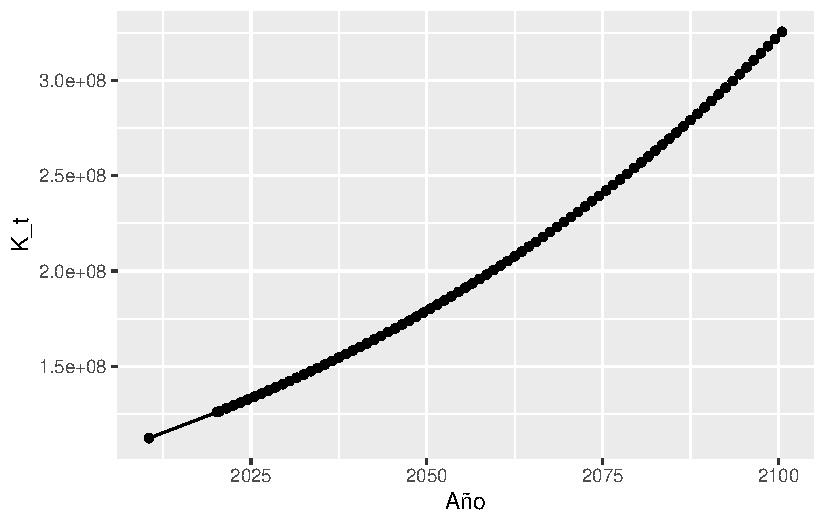
\includegraphics[keepaspectratio]{Trabajo-Final-9219_files/figure-pdf/unnamed-chunk-4-1.pdf}}

\begin{Shaded}
\begin{Highlighting}[]
\CommentTok{\#tasas brutas y especificas}
\NormalTok{deaths}\OtherTok{\textless{}{-}}\NormalTok{deaths }\SpecialCharTok{\%\textgreater{}\%}
  \FunctionTok{mutate}\NormalTok{(}\AttributeTok{m\_x=}\NormalTok{ D}\SpecialCharTok{/}\NormalTok{ N)}

\FunctionTok{plot}\NormalTok{(deaths[location}\SpecialCharTok{==} \StringTok{"Argentina"}\NormalTok{,x], }\FunctionTok{log}\NormalTok{(deaths[location }\SpecialCharTok{==} \StringTok{"Argentina"}\NormalTok{,m\_x]))}
\end{Highlighting}
\end{Shaded}

\pandocbounded{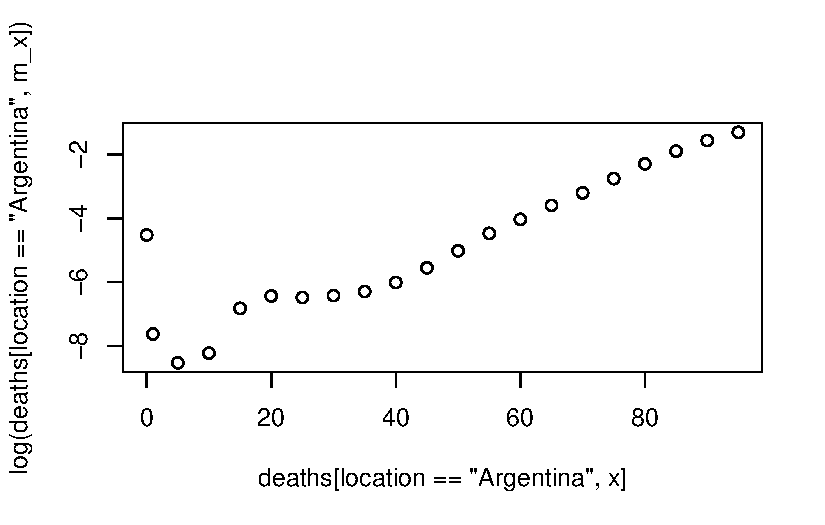
\includegraphics[keepaspectratio]{Trabajo-Final-9219_files/figure-pdf/unnamed-chunk-5-1.pdf}}

\begin{Shaded}
\begin{Highlighting}[]
\CommentTok{\#tasa bruta de mortalidad}
\NormalTok{deaths }\SpecialCharTok{\%\textgreater{}\%}
  \FunctionTok{group\_by}\NormalTok{(location) }\SpecialCharTok{\%\textgreater{}\%}
  \FunctionTok{summarise}\NormalTok{(}\FunctionTok{weight\_mean}\NormalTok{(m\_x, x }\SpecialCharTok{/} \FunctionTok{sum}\NormalTok{(x)))}
\end{Highlighting}
\end{Shaded}

\begin{verbatim}
# A tibble: 2 x 2
  location  `weight_mean(m_x, x/sum(x))`
  <chr>                            <dbl>
1 Argentina                       0.0814
2 Guatemala                       0.103 
\end{verbatim}

\begin{Shaded}
\begin{Highlighting}[]
\NormalTok{mort }\OtherTok{\textless{}{-}} \FunctionTok{fread}\NormalTok{(}\StringTok{"https://population.un.org/wpp/assets/Excel\%20Files/1\_Indicator\%20(Standard)/CSV\_FILES/WPP2024\_DeathsBySingleAgeSex\_Medium\_1950{-}2023.csv.gz"}\NormalTok{)}

\NormalTok{APV }\OtherTok{\textless{}{-}} \FunctionTok{fread}\NormalTok{(}\StringTok{"https://population.un.org/wpp/assets/Excel\%20Files/1\_Indicator\%20(Standard)/CSV\_FILES/WPP2024\_PopulationBySingleAgeSex\_Medium\_1950{-}2023.csv.gz"}\NormalTok{)}

\DocumentationTok{\#\# LocID 484 México y 392 Japón}
\end{Highlighting}
\end{Shaded}

\begin{Shaded}
\begin{Highlighting}[]
\NormalTok{ruta\_archivo }\OtherTok{\textless{}{-}} \StringTok{"C:/Users/Mario Escobar/Downloads/Ciencias/Demografia/Demography\_9219/Demography\_9219/data/Tabla mort\_guatemala.xlsx"}

\NormalTok{guatemala }\OtherTok{\textless{}{-}} \FunctionTok{read\_excel}\NormalTok{(ruta\_archivo, }
                        \AttributeTok{sheet =} \StringTok{"tabla mortalidad 1998"}\NormalTok{,}
                        \AttributeTok{skip =} \DecValTok{2}
\NormalTok{                        )}\SpecialCharTok{\%\textgreater{}\%}
  
  \FunctionTok{rename\_with}\NormalTok{(}\SpecialCharTok{\textasciitilde{}}\FunctionTok{case\_when}\NormalTok{(}
\NormalTok{    .x }\SpecialCharTok{\%in\%} \FunctionTok{c}\NormalTok{(}\StringTok{"x"}\NormalTok{, }\StringTok{"x (edad)"}\NormalTok{) }\SpecialCharTok{\textasciitilde{}} \StringTok{"x"}\NormalTok{,}
\NormalTok{    .x }\SpecialCharTok{\%in\%} \FunctionTok{c}\NormalTok{(}\StringTok{"nKx"}\NormalTok{, }\StringTok{"K"}\NormalTok{) }\SpecialCharTok{\textasciitilde{}} \StringTok{"K"}\NormalTok{,}
\NormalTok{    .x }\SpecialCharTok{\%in\%} \FunctionTok{c}\NormalTok{(}\StringTok{"nDx"}\NormalTok{, }\StringTok{"D"}\NormalTok{) }\SpecialCharTok{\textasciitilde{}} \StringTok{"D"}\NormalTok{,}
    \ConstantTok{TRUE} \SpecialCharTok{\textasciitilde{}}\NormalTok{ .x}
\NormalTok{  ))}\SpecialCharTok{\%\textgreater{}\%}

  \FunctionTok{mutate}\NormalTok{(}
    \AttributeTok{x =} \FunctionTok{as.numeric}\NormalTok{(x),}
    \AttributeTok{n =} \FunctionTok{as.numeric}\NormalTok{(n),}
    \AttributeTok{K =} \FunctionTok{as.numeric}\NormalTok{(K),}
    \AttributeTok{D =} \FunctionTok{as.numeric}\NormalTok{(D),}
    
    \AttributeTok{mx =}\NormalTok{ D}\SpecialCharTok{/}\NormalTok{K }\CommentTok{\#tasa mortalidad}
\NormalTok{  )}
\end{Highlighting}
\end{Shaded}

\begin{verbatim}
New names:
* `nMx` -> `nMx...5`
* `ndx` -> `ndx...10`
* `nMx` -> `nMx...14`
* `` -> `...16`
* `` -> `...17`
* `` -> `...18`
* `ndx` -> `ndx...19`
\end{verbatim}

\begin{verbatim}
Warning: There was 1 warning in `mutate()`.
i In argument: `x = as.numeric(x)`.
Caused by warning:
! NAs introducidos por coerción
\end{verbatim}

\begin{Shaded}
\begin{Highlighting}[]
\CommentTok{\#funcion tablas de vida}

\NormalTok{lt\_abr }\OtherTok{\textless{}{-}} \ControlFlowTok{function}\NormalTok{(x, n, mx, }\AttributeTok{sex =} \StringTok{"f"}\NormalTok{, }\AttributeTok{IMR =} \ConstantTok{NA}\NormalTok{)\{}
\NormalTok{  m }\OtherTok{\textless{}{-}} \FunctionTok{length}\NormalTok{(x)}
\NormalTok{  ax }\OtherTok{\textless{}{-}}\NormalTok{ n}\SpecialCharTok{/}\DecValTok{2}
  
  \CommentTok{\#ajuste coale{-}demeny para 0{-}1}
  \ControlFlowTok{if}\NormalTok{(sex }\SpecialCharTok{==} \StringTok{"m"}\NormalTok{)\{}
\NormalTok{    ax[}\DecValTok{1}\NormalTok{] }\OtherTok{\textless{}{-}} \FunctionTok{ifelse}\NormalTok{(mx[}\DecValTok{1}\NormalTok{] }\SpecialCharTok{\textgreater{}=} \FloatTok{0.107}\NormalTok{, }\FloatTok{0.330}\NormalTok{, }\FloatTok{0.45+2.684}\SpecialCharTok{*}\NormalTok{mx[}\DecValTok{1}\NormalTok{])}
\NormalTok{  \}}\ControlFlowTok{else}\NormalTok{\{}
\NormalTok{    ax[}\DecValTok{1}\NormalTok{] }\OtherTok{\textless{}{-}} \FunctionTok{ifelse}\NormalTok{(mx[}\DecValTok{1}\NormalTok{]}\SpecialCharTok{\textgreater{}=}\FloatTok{0.107}\NormalTok{,}\FloatTok{0.350}\NormalTok{, }\FloatTok{0.053+2.800}\SpecialCharTok{*}\NormalTok{mx[}\DecValTok{1}\NormalTok{])}
\NormalTok{  \}}
  
  \CommentTok{\#ajuste para 1{-}4}
  
   \ControlFlowTok{if}\NormalTok{(sex }\SpecialCharTok{==} \StringTok{"m"}\NormalTok{)\{}
\NormalTok{    ax[}\DecValTok{2}\NormalTok{] }\OtherTok{\textless{}{-}} \FunctionTok{ifelse}\NormalTok{(mx[}\DecValTok{1}\NormalTok{] }\SpecialCharTok{\textgreater{}=} \FloatTok{0.107}\NormalTok{, }\FloatTok{1.352}\NormalTok{, }\FloatTok{1.651+2.816}\SpecialCharTok{*}\NormalTok{mx[}\DecValTok{1}\NormalTok{])}
\NormalTok{  \}}\ControlFlowTok{else}\NormalTok{\{}
\NormalTok{    ax[}\DecValTok{2}\NormalTok{] }\OtherTok{\textless{}{-}} \FunctionTok{ifelse}\NormalTok{(mx[}\DecValTok{1}\NormalTok{]}\SpecialCharTok{\textgreater{}=}\FloatTok{0.107}\NormalTok{,}\FloatTok{1.361}\NormalTok{, }\FloatTok{1.522+1.518}\SpecialCharTok{*}\NormalTok{mx[}\DecValTok{1}\NormalTok{])}
\NormalTok{  \} }
  
  \CommentTok{\#proba de morir}
  
\NormalTok{  qx }\OtherTok{\textless{}{-}}\NormalTok{ (n}\SpecialCharTok{*}\NormalTok{mx)}\SpecialCharTok{/}\NormalTok{(}\DecValTok{1}\SpecialCharTok{+}\NormalTok{(n}\SpecialCharTok{{-}}\NormalTok{ax)}\SpecialCharTok{*}\NormalTok{mx)}
\NormalTok{  qx[m] }\OtherTok{\textless{}{-}} \DecValTok{1}
  
  \CommentTok{\#proba supervivencia}
  
\NormalTok{  px }\OtherTok{\textless{}{-}} \DecValTok{1}\SpecialCharTok{{-}}\NormalTok{qx}
  
  \CommentTok{\#lx}
  
\NormalTok{  lx }\OtherTok{\textless{}{-}} \DecValTok{100000} \SpecialCharTok{*} \FunctionTok{cumprod}\NormalTok{(}\FunctionTok{c}\NormalTok{(}\DecValTok{1}\NormalTok{, px[}\SpecialCharTok{{-}}\NormalTok{m]))}
  
  \CommentTok{\#dx}
  
\NormalTok{  dx }\OtherTok{\textless{}{-}} \FunctionTok{c}\NormalTok{(}\SpecialCharTok{{-}}\FunctionTok{diff}\NormalTok{(lx),lx[m])}
  
  \CommentTok{\#Lx}
  
\NormalTok{  Lx }\OtherTok{\textless{}{-}}\NormalTok{ n}\SpecialCharTok{*}\FunctionTok{c}\NormalTok{(lx[}\SpecialCharTok{{-}}\DecValTok{1}\NormalTok{],}\DecValTok{0}\NormalTok{) }\SpecialCharTok{+}\NormalTok{ ax}\SpecialCharTok{*}\NormalTok{dx}
\NormalTok{  Lx[m] }\OtherTok{\textless{}{-}}\NormalTok{ lx[m]}\SpecialCharTok{/}\NormalTok{mx[m]}
  
  \CommentTok{\#Tx}
  
\NormalTok{  Tx }\OtherTok{\textless{}{-}} \FunctionTok{rev}\NormalTok{(}\FunctionTok{cumsum}\NormalTok{(}\FunctionTok{rev}\NormalTok{(Lx)))}
  
  \CommentTok{\#e\_x}
  
\NormalTok{  ex }\OtherTok{\textless{}{-}}\NormalTok{ Tx}\SpecialCharTok{/}\NormalTok{lx}
  
  \FunctionTok{return}\NormalTok{(}\FunctionTok{data.table}\NormalTok{(x, n, mx, ax, qx, px, lx, dx, Lx, Tx, ex))}
\NormalTok{\}}

\NormalTok{tabla\_vida\_1998 }\OtherTok{\textless{}{-}} \FunctionTok{lt\_abr}\NormalTok{(}\AttributeTok{x =}\NormalTok{ guatemala}\SpecialCharTok{$}\NormalTok{x, }\AttributeTok{n=}\NormalTok{ guatemala}\SpecialCharTok{$}\NormalTok{n, }\AttributeTok{mx =}\NormalTok{ guatemala}\SpecialCharTok{$}\NormalTok{mx, }\AttributeTok{sex =} \StringTok{"f"}\NormalTok{)}
\FunctionTok{print}\NormalTok{(tabla\_vida\_1998)}
\end{Highlighting}
\end{Shaded}

\begin{verbatim}
        x     n           mx        ax          qx        px        lx
    <num> <num>        <num>     <num>       <num>     <num>     <num>
 1:     0     1 0.0368534518 0.1561897 0.035741972 0.9642580 100000.00
 2:     1     4 0.0056623841 1.5779435 0.022343109 0.9776569  96425.80
 3:     5     5 0.0008990908 2.5000000 0.004485372 0.9955146  94271.35
 4:    10     5 0.0007038573 2.5000000 0.003513105 0.9964869  93848.51
 5:    15     5 0.0010193168 2.5000000 0.005083630 0.9949164  93518.81
 6:    20     5 0.0014609051 2.5000000 0.007277944 0.9927221  93043.39
 7:    25     5 0.0018931032 2.5000000 0.009420929 0.9905791  92366.23
 8:    30     5 0.0023472145 2.5000000 0.011667607 0.9883324  91496.05
 9:    35     5 0.0028750333 2.5000000 0.014272581 0.9857274  90428.51
10:    40     5 0.0036333321 2.5000000 0.018003132 0.9819969  89137.87
11:    45     5 0.0047615176 2.5000000 0.023527521 0.9764725  87533.10
12:    50     5 0.0069539413 2.5000000 0.034175569 0.9658244  85473.67
13:    55     5 0.0100253246 2.5000000 0.048901002 0.9510990  82552.56
14:    60     5 0.0157206624 2.5000000 0.075630893 0.9243691  78515.65
15:    65     5 0.0221879713 2.5000000 0.105109443 0.8948906  72577.44
16:    70     5 0.0328469895 2.5000000 0.151771828 0.8482282  64948.87
17:    75     5 0.0575430391 2.5000000 0.251530607 0.7484694  55091.46
18:    80     5 0.1012608546 2.5000000 0.404024586 0.5959754  41234.27
19:    NA    NA 0.1747496735        NA 1.000000000 0.0000000  24574.61
            dx        Lx        Tx        ex
         <num>     <num>     <num>     <num>
 1:  3574.1972  96984.06 6974043.5 69.740435
 2:  2154.4523 380485.01 6877059.4 71.319701
 3:   422.8421 470299.65 6496574.4 68.913561
 4:   329.6996 468418.29 6026274.8 64.212792
 5:   475.4150 466405.51 5557856.5 59.430360
 6:   677.1646 463524.06 5091451.0 54.721252
 7:   870.1757 459655.71 4627926.9 50.104102
 8:  1067.5400 454811.42 4168271.2 45.556842
 9:  1290.6483 448915.95 3713459.8 41.065143
10:  1604.7608 441677.42 3264543.9 36.623536
11:  2059.4370 432516.93 2822866.4 32.249130
12:  2921.1112 420065.56 2390349.5 27.965917
13:  4036.9027 402670.52 1970283.9 23.867025
14:  5938.2090 377732.75 1567613.4 19.965616
15:  7628.5748 343815.79 1189880.7 16.394634
16:  9857.4087 300100.83  846064.9 13.026630
17: 13857.1886 240814.33  545964.1  9.910139
18: 16659.6598 164522.21  305149.7  7.400391
19: 24574.6126 140627.52  140627.5  5.722471
\end{verbatim}

\begin{Shaded}
\begin{Highlighting}[]
\CommentTok{\#grafica}

\FunctionTok{ggplot}\NormalTok{(tabla\_vida\_1998, }\FunctionTok{aes}\NormalTok{(}\AttributeTok{x=}\NormalTok{x, }\AttributeTok{y=}\NormalTok{mx)) }\SpecialCharTok{+} \FunctionTok{geom\_line}\NormalTok{(}\AttributeTok{color =}\StringTok{"violet"}\NormalTok{) }\SpecialCharTok{+}
\FunctionTok{scale\_y\_log10}\NormalTok{() }\SpecialCharTok{+} \FunctionTok{theme\_minimal}\NormalTok{() }\SpecialCharTok{+} \FunctionTok{labs}\NormalTok{(}\AttributeTok{title =} \StringTok{"Tasa de mortalidad {-} Escala log"}\NormalTok{,}
                                         \AttributeTok{x =}\StringTok{"Edad"}\NormalTok{,}
                                         \AttributeTok{y =} \StringTok{"mx log"}\NormalTok{)}
\end{Highlighting}
\end{Shaded}

\begin{verbatim}
Warning: Removed 1 row containing missing values or values outside the scale range
(`geom_line()`).
\end{verbatim}

\pandocbounded{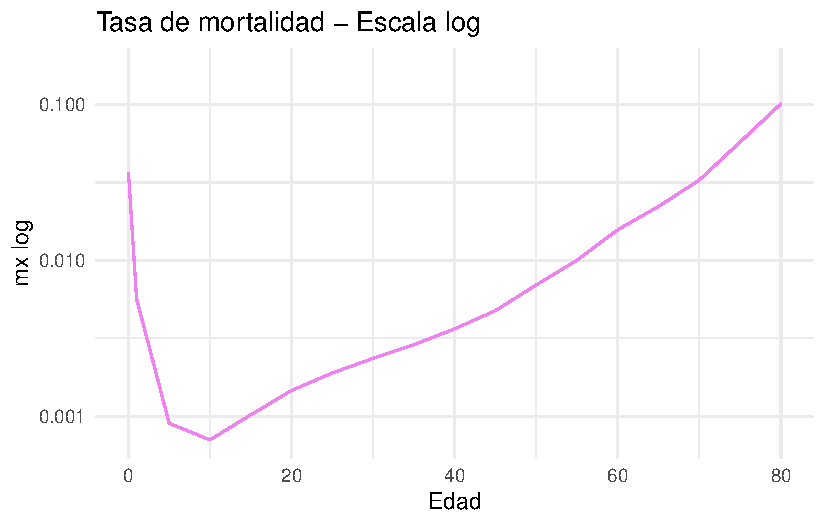
\includegraphics[keepaspectratio]{Trabajo-Final-9219_files/figure-pdf/unnamed-chunk-8-1.pdf}}




\end{document}
